
\begin{figure*}
	\centering
	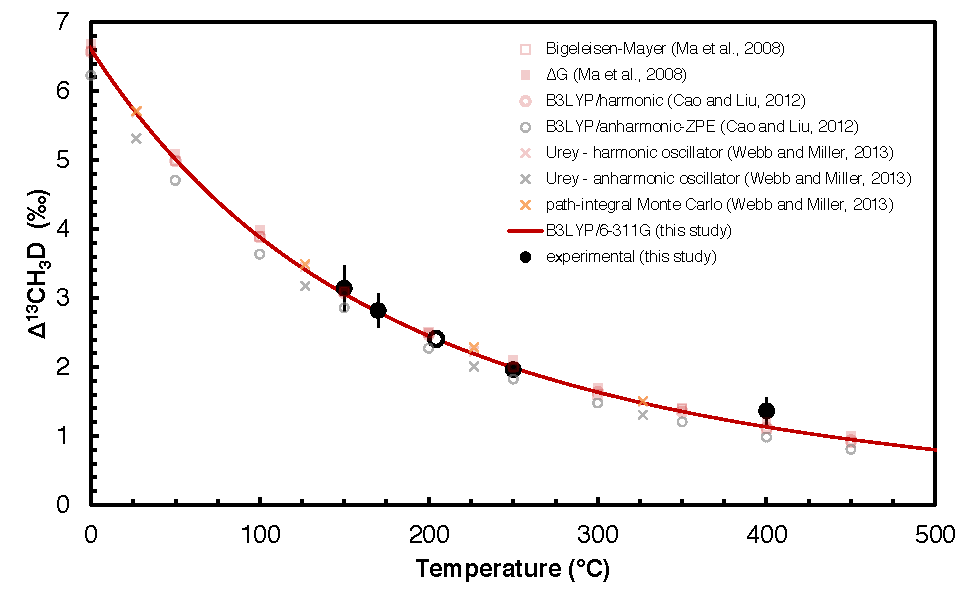
\includegraphics[width=0.8\linewidth]{figures/Fig2.S1}
	\caption[Experimental calibration of the
	Δ\textsuperscript{13}CH\textsubscript{3}D thermometer]{Experimental calibration of the
		Δ\textsuperscript{13}CH\textsubscript{3}D thermometer. Filled circles
	represent the mean Δ\textsuperscript{13}CH\textsubscript{3}D of gases
	heated at that temperature, and error bars represent 95\% confidence
	intervals calculated from a normal distribution (for the 150~°C sample,
	error bars represent the 95\% confidence interval on the measurement
	cycles in a single analysis, calculated from a \emph{t}-distribution).
	For the 250~°C point, the error bars are smaller than the symbol. The
	open circle represents our reference gas, AL1. The equilibrium curve
	(red line) was calculated following conventional equilibrium isotope
	fractionation theory under the harmonic oscillator assumption
	\parencite{Bigeleisen+Mayer_1947_JCP}; frequencies were calculated at the B3LYP level of theory
	using the 6-311G basis set as implemented in Gaussian 03 (\citeauthor{g03}).
	For comparison, results from published computational studies
	\parencite{Webb+Miller_2013_JPCA,Cao+Liu_2012_GCA,Ma++_2008_GCA} are also plotted.}
	\label{fig:2:S1}
\end{figure*}